\chapter{Design} \label{section:design}
In the spirit of an extensive overview of standardized procedures of industrial vibration acquisition and monitoring, the methods in feature selection, feature selection, and machine diagnostics from vibration signals, we propose a preliminary design of elements in the sensor network capable of discriminating machinery faults.

\section{Preparatory exploration}
The wood processing factory we plan to collaborate with has to choose machines that are worthy of condition monitoring. In the meantime, the data processing pipeline will be put together in Python language and packages for scientific computing. The pipeline will consist of the following stages.

\begin{enumerate}
    \itemsep0pt
    \item Detrending
    \item Adaptive noise cancellation of the background interference
    \item Vector of all features
    \begin{itemize}
        \itemsep0pt
        \item Time domain: statistical measures (Tab.~\ref{tab:td-features})
        \item Frequency domain: PSD estimation with FFT and Welch averaging with the resolution of 1 Hz combined with Hann window (Tab.~\ref{tab:fd-features})
        \item Time-frequency domain: energy and entropy in wavelet coefficients from WPD and EWT filter banks.
    \end{itemize}
    \item Feature selection on evaluation datasets and experimental measurements from the factory to prune away irrelevant features with pearson correlation, Fisher score, and mutal information.
    \item Model evaluation and comparison of novelty detection methods and precision of classification with different sets of predictors. The range of optimal parameters will be found for the DenStream ($\mu$, $\epsilon$, $beta$, $\lambda$), Half-Space Trees (window size, ensemble size), and kNN (distance metric, $k$ neighbours). Evaluation metrics associated with confusion matrices will be used like accuracy, precision, true positive rate, and false positive rate.
\end{enumerate}

\begin{figure}[h]
\centering
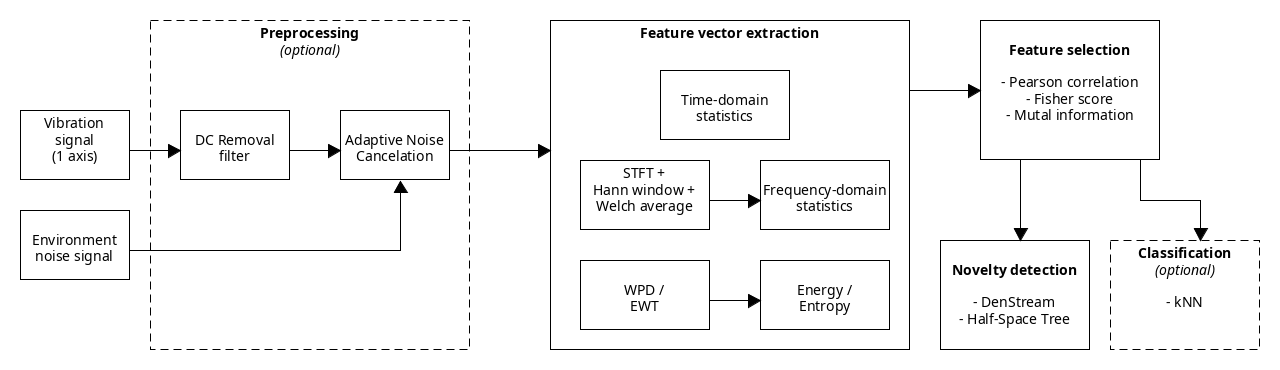
\includegraphics[width=0.9\textwidth]{assets/ml-lifecycle.png}
\caption{Machine learning lifecycle of feature discovery}
\end{figure}


\section{Measurment strategy}
Describe technical inspection in VNET, a.s. datacentres (DC Digitalis, SHC\rom{2}) from 12th October 2023
and 

HVAC - Air conditioning, Refrigirator
Devices:
	- Adiabatic plunger pump: better candidates because of fraquent faults, datacentere is inspected daily and maintaned regulary so it is not that critical, turns off under 26°C to save electricity consumption in winter, we do not have faulty machines for comparision
	
	- Scroll compressor: example Copeland ZR16M3E-TWD-561 (2900 RPM @ 50 Hz; 9,7 kW (13 HP); 380/420V; 25 A) 3500 RPM @ 60Hz
	
	Faults (\url{https://www.mdpi.com/1099-4300/17/10/7076})
	- unbalance of the rotor, fault of the scroll, mechanical assembly loose, bearing loose
	
	- Fig: insert image of cut of compressor
	- Fig: insert spectrograms, orbitals from exploratory measurements
	
- How to obtain dataset (plan had to been aggreed to by datacentre technician)
 	- every 2 or 3 weeks (4 - 6 times)
 	- 60 - 90 s recordings in each place
  	- good and bad compressor (4 x top, 4x side, 1x base)
	
	
\section{Embedded system for dataset measurement}	
Functional requirements
\begin{itemize}
	\item MCU has interface to accept commands and storage to save measurements
	\item Driver for accelerometer is build in
	\item Accelerometer has frequency response at least 500 Hz (FS = min. 3200 Hz)
\end{itemize}
Business (management) requirements: because of time constraints before first technical inspection: build from parts already on stock or inexpensive and quickly procurable, driver should be available, easily save massive recordings to persistant storage, extensible platform in case better option would not be avaiable in the future

Hardware parts:
Faster than target device to enable experimentation, ARM platform
\begin{itemize}
	\item Beaglebone Black 
		(Texas Instruments Sitara AM3358: 1GHz ARM Cortex-A8, 
		 SDRAM: 512MB DDR3L 800MHZ, 
		 Onboard Flash: 4GB)
	\item OS: Debian 10 Kernel 5.10.168-ti-r72
	\item Accelerometer ADXL335, 3-Axis $\pm$3 g Accelerometer, 
	      Bandwidths X, Y axes: (0.5 Hz - 1.6 kHz), Z axes: (0.5 Hz - 0.55 kHz)
	  (via 8 channel 12-bit SAR ADC, 1.8V, 200 MSPS)
	 \item Later: ADXL345 (SPI, ODR: 3.2 kHz) 
\end{itemize}

\section{Vibration processing}
 \begin{itemize}
 \itemsep0pt
\item \textbf{Input:} Samples from three-axis MEMS accelerometers, RPM tachometer, Noise background
\item \textbf{Output:} machine health status / type of fault
\item \textbf{Output on demand}: Control chart of trend features
\end{itemize}

\begin{enumerate}
\itemsep0pt
\item \textbf{Accelerometer} - MEMS accelerometers will be placed on at least two distinct measurement points in two perpendicular axes and one sensor in the machine base for denoising purposes. Rotational speed has to be captured at the same time too. The sampling frequency shall be around 2 kHz if unbalance and looseness is to be identified, and 10 kHz if bearing faults are also of interest. The range of overall rms vibrations is not expected to exceed 30 mm/s according to the vibration severity chart.
\item \textbf{Acquisition interval} - sensor units will be triggered in regular intervals (every 15 - 60 minutes) to collect vibration recordings from the band saw (or another machine of choice). The machine has to be under the same load conditions every time is recording is active. 
\item \textbf{Features} - most relevant features are computed and compared to recent measurements. If there is a statistically significant change the whole summary is sent, otherwise keep-alive notification is sent. 
\item \textbf{Wireless network} - earlier design decision has been made to establish wireless connections. Therefore, the sensor unit will send data over Wifi (IEEE 802.11), or Thread with IEEE 802.15.4 over 2.4 GHz or 868 MHz frequency bands. The application protocol shall be Constrained Application Protocol (CoAP). The messages will be encoded by Concise Binary Object Representation (CBOR) or MessagePack which provides the best compression ratio and is widely supported.
\item \textbf{Time series database} - stores history of trend values. Raw vibration measurements can be requested by the operator at any time but are available and delayed according to transfer speeds and other network constraints. The promissing database technologies is TimescaleDB.
\item \textbf{Diagnosis panel} - continuously updates the anomaly detection and classification models with the introduction of annotations to notify the operator about observed faults and imminent failure of the machine. The dashboard is provided to display the current status of multiple machines.
\end{enumerate}

\begin{figure}[h]
\centering
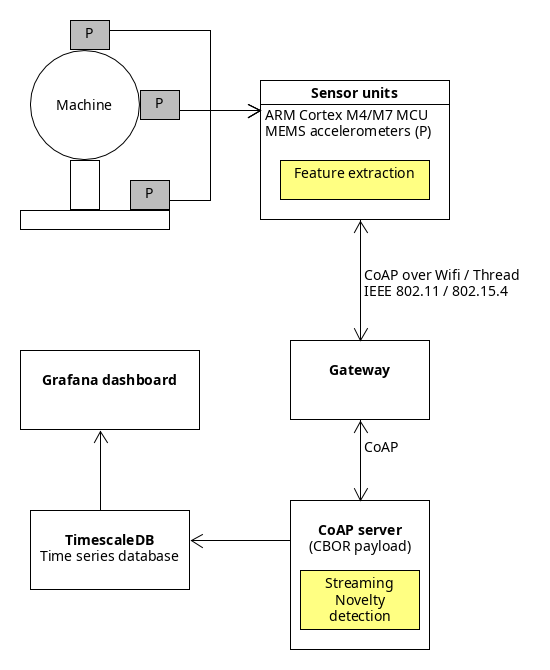
\includegraphics[width=0.7\textwidth]{assets/sensor-network.png}
\caption{Sensor network components}
\end{figure}


\chapter{ML Pipeline Design}

Mafaulda dataset
Jupyter notebook - Python


\section{Data labeling and cleaning}
- Mafaulda labeling and creating subset (RPM range, 4 classes, Anomaly class)
- Measurement of custom datasets (Schiratech iComox, Beaglebone) - air conditioning, compressor

\section{Feature relevance}
- supervised - correlation, fisher, mi
- custom, tsfel, in sensor and in one axis
- online learning features

\section{Nearest neighbour classifier}
- kNN (fault and anomaly)
	- Offine (baseline)
	- Online (evolution)
- parameters: k-neigh, distance
- metrics: accuracy, precision, recall

\section{Clustering}
- Density based clustering
	- DBSCAN (all features, PCA, subset of best)
	- DenStream (all features, subset of best)

\section{Anomaly detection / Decision Trees}
- Offline (DecisionTree)
- Online (Hoefing Tree)

\section{Comparision to real data}
- Can be part of original chapters
